\documentclass{beamer}
\usetheme{Madrid}

\title{Detecting Medication Dosing Errors in Clinical Trial Protocols}
\subtitle{A Multimodal Machine Learning Approach}
\author{BioNLP Project}
\date{\today}

\begin{document}

\begin{frame}
\titlepage
\end{frame}

\begin{frame}{Why This Matters}
\begin{itemize}
\item Medication dosing errors can lead to patient harm, trial delays, and increased costs.
\item Clinical trial protocols contain both structured metadata and biomedical text.
\item Manual review is expensive and time-consuming.
\item BioNLP enables automatic identification of high-risk protocols before trials begin.
\end{itemize}
\end{frame}

\begin{frame}{The Challenge}
\begin{itemize}
\item Identify protocols with high inherent risk of dosing errors.
\item CT-DEB dataset: $>$42,000 clinical trial narratives.
\item Binary classification task.
\item Severe class imbalance: only $\sim$5\% positive examples.
\end{itemize}
\end{frame}

\begin{frame}{Dataset Overview}
\begin{itemize}
\item Source: CT-Dosing-Errors-Benchmark (CT-DEB)
\item ClinicalTrials.gov protocols
\item $>$42,000 trial narratives
\item Positive class: reported dosing error
\item Negative class: no reported dosing error
\end{itemize}
\end{frame}

\begin{frame}{Our Approach}
\textbf{Structured Data Branch}
\begin{itemize}
\item Metadata extraction
\item Optimized XGBoost classifier
\end{itemize}

\textbf{Biomedical NLP Branch}
\begin{itemize}
\item Aggregated protocol text
\item Fine-tuned PubMedBERT
\item Binary classification
\end{itemize}
\end{frame}

\begin{frame}{Modality Fusion}
\textbf{Late Fusion}
\begin{itemize}
\item Average predictions from XGBoost and PubMedBERT
\end{itemize}

\textbf{Early Fusion}
\begin{itemize}
\item Extract PubMedBERT embeddings
\item Concatenate with metadata
\item Train unified XGBoost model
\end{itemize}
\end{frame}

\begin{frame}{Results}
\begin{columns}
\begin{column}{0.4\textwidth}
\begin{table}
\resizebox{\textwidth}{!}{%
\begin{tabular}{lcc}
\hline
Model & ROC-AUC & F1 \\
\hline
Text-Only & 0.8210 & 0.2526 \\
Stats-Only & 0.8466 & 0.2972 \\
Early-Fusion & 0.8475 & 0.2904 \\
Late-Fusion & \textbf{0.8486} & \textbf{0.3112} \\
\hline
\end{tabular}%
}
\end{table}
\end{column}
\begin{column}{0.6\textwidth}
\centering
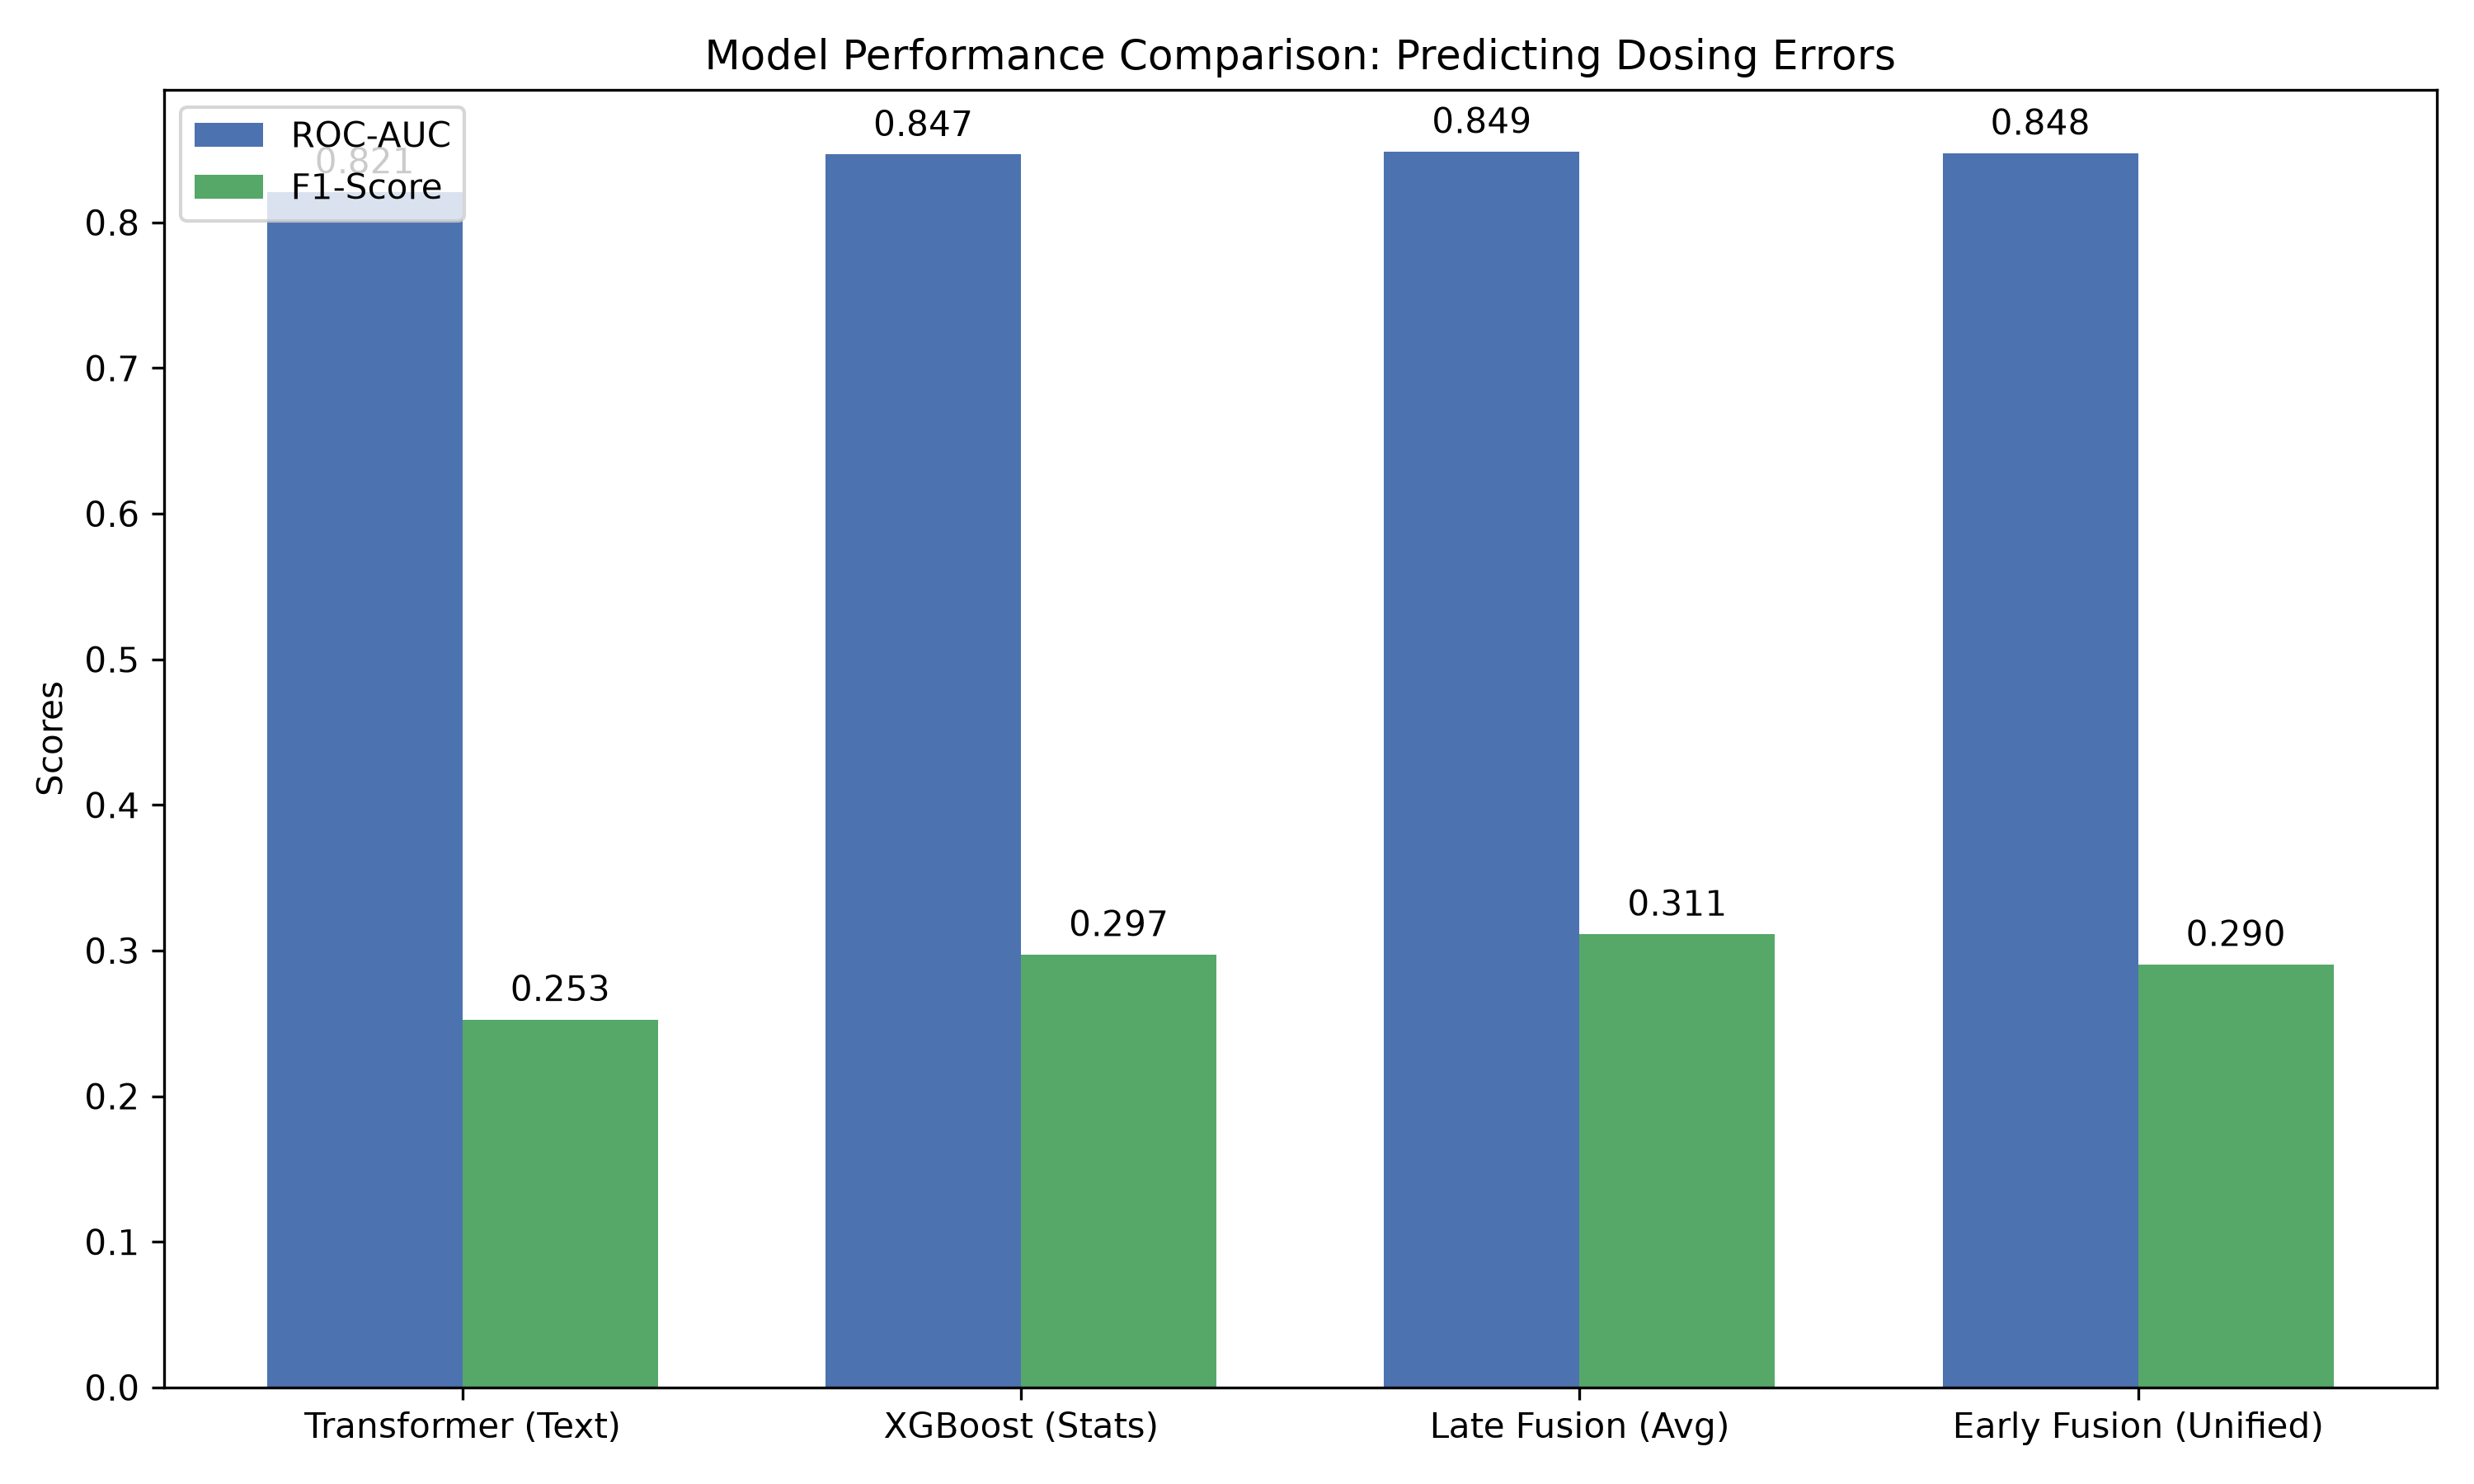
\includegraphics[width=\textwidth]{model_comparison.png}
\end{column}
\end{columns}
\end{frame}

\begin{frame}{Feature Impact}
\begin{columns}
\begin{column}{0.5\textwidth}
\textbf{Key Drivers of Risk:}
\begin{enumerate}
\item Trial Phase (Phase 4)
\item Enrollment Count
\item Number of Locations
\end{enumerate}
\vspace{0.5cm}
Larger, multi-center, post-marketing trials inherently possess much higher statistical likelihoods of administrative dosing errors.
\end{column}
\begin{column}{0.5\textwidth}
\centering

\includegraphics[width=\textwidth]{feature_importance.png}
\end{column}
\end{columns}
\end{frame}

\begin{frame}{Conclusions}
\begin{itemize}
\item Structured metadata outperformed text-only modeling.
\item Fusion improved predictive performance.
\item Early fusion showed limited gains due to the curse of dimensionality.
\item Late fusion achieved the best overall results.
\end{itemize}
\end{frame}

\begin{frame}{Future Work}
\begin{itemize}
\item Compare BioBERT, ClinicalBERT, and PubMedBERT
\item Expand SHAP explainability analysis
\item Explore LLM Zero-shot Prompting for feature extraction
\item Extension to other clinical trial safety tasks
\end{itemize}
\end{frame}

\begin{frame}
\centering
\Huge Questions?
\end{frame}

\end{document}
